\chapter{Arquitectura y modelo de datos}
\label{cap:modeloDeDatos}
En este capítulo se explicará la arquitectura y el modelo de datos utilizado en la aplicación. 

En la sección de arquitectura se explicará la arqitectura seguida en el proyecto, así como los patrones utilizados. Por otro lado, en la sección de modelo de datos, se hará una descripición de todas las estructuras de datos utilizadas, explicándolas brevemente para dar un poco de contexto, sin embargo, siempre se recomienda ver y tocar el código para entenderlo en profundidad. En segundo lugar se explicarán todos los servicios utilizados para mantener la persistencia: Firebase (principal herramienta utilizada como \textit{backend}), Datastore (se ha utilizado para guardar en local preferencias del sistema) y por último se explicará como se ha utilizado el patrón Singleton para evitar tener que usar una base de datos local como 
Room\hyperlink{cap:biblio}{\endnote{\textbf{Room}: \url{https://developer.android.com/training/data-storage/room/}}}, logrando así una aplicación completa que pueda interactuar con otros dispositivos a través de la red.
\section{Arquitectura y patrones}
\subsection{CLEAN architecture}
\label{subsec:cleanArch}
La arquitectura CLEAN, originaria del libro \textit{Clean Architecture} (Martin, 2017)\hyperlink{cap:biblio}{\endnote{
\textit{Clean Architecture: A Craftsman's Guide to Software Structure and Design}, Robert C. Martin, 2017}}, es una forma de estructurar el software, dividiendolo en distintas capas que abstraigan el código y separen responsabilidades. Gracias al uso de esta arquitectura, se ha podido crear un proyecto escalable y robusto. También se han ahorrado muchos dolores de cabeza en los distintos procesos de refactorización ya que al haber tenido una estructura ordenada y bien definida, se han evitado posibles efectos secundarios por causa de los distintos cambios.

En Profinder se ha adaptado esta arquitectura a la programación en Android, dividiéndose así el código en cuatro capas explicadas a continuación:
\begin{enumerate}
    \item core: en esta capa van los recursos comunes que pueden ser accedidos por todas las demás capas, esta es una relación unidireccional ya que core no puede acceder a las demás capas. En este proyecto en particular se ha utilizado para guardar todo el boilerplate necesario para la aplicación del MVI (explicado en la apartado \ref{subsec:mvi}), modelos de datos para pruebas, y utilidades como la clase encargada de formatear las fechas y combinar los identificadores de usuarios.
    \item data: en esta capa es donde se gestionan todos los servicios y se preparan para ser enviados a la capa domain (explicada en el siguiente punto). Esta capa tiene toda la lógica de aplicación y es la encargada de decidir de dónde sacar los datos, todas las llamadas de red se hacen en esta capa. En muchos casos, esta capa tiene un modelo de datos propio (los datos tal cual llegan de los \textit{endpoints}) que adapta mediante el uso de \textit{mappers} para ser enviados a la siguiente capa.
    \item domain: En esta capa se encuentra la lógica de negocio de la aplicación, sería común a todas las versiones de la aplicación si se hicieran para otros sistemas operativos (IOS, Windows...) a excepción de la adecuación con el lenguaje de programación específico de cada sistema operativo, esto significa que no le ‘importa’ de donde vienen los datos, cuenta con una interfaz (denominada repositorio) en la que se ha definido el contrato con la capa de data y es ahí donde pide los datos que le deben llegar según su propio modelo (mapeados). Es en esta capa donde se definen los casos de uso, que actúan como contratos entre la capa de UI (explicada en el siguiente punto) y el repositorio. Esta implementación abstrae responsabilidades y ayuda a la encapsulación. 
    \item ui: Esta es toda la capa de interfaz de usuario de la aplicación, realizada utilizando \hyperlink{subsec:compose}{Jetpack compose} y siguiendo el patrón arquitectónico  MVI (\ref{subsec:mvi}). Las vistas como tal (denominadas \textit{Composables}) se comunican con los casos de uso (capa domain) a través de unas clases denominadas \textit{Viewmodels}\hyperlink{cap:biblio}{\endnote{\textbf{Viewmodels}: \url{https://developer.android.com/topic/libraries/architecture/viewmodel}}}.
\end{enumerate}

\hypertarget{subsec:mvi}{}
\subsection{MVI}
\label{subsec:mvi}
Debido a que en una aplicación móvil la mayor parte del trabajo se realiza en la interfaz de usuario, es habitual seguir patrones de diseño (mejor denominados: pseudo-arquitecturas). En el caso de Profinder había dos posibilidades: MVVM\hyperlink{cap:biblio}{\endnote{\textbf{MVVM}: \url{https://builtin.com/software-engineering-perspectives/mvvm-architecture}}} (Model-View-Viewmodel) o MVI (Model-View-Intent). Se decidió seguir el patrón MVI por ser más organizado y viable para aplicaciones de tamaño grande, a su vez es un patrón que se adapta muy bien al paradigma de programación en kotlin (programación funcional), su única desventaja es que introduce código de relleno para la estructuración (denominado boilerplate), pero esto a su vez ayuda a que sea más entendible por terceros a medida que aumenta el tamaño del proyecto. A continuación se explica en qué consiste esta pseudo-arquitectura y como se ha aplicado en el proyecto:
\begin{itemize}
    \item \textbf{Model}: es un término que puede variar en distintas pseudo-arquitecturas, en MVI es el que representa el estado de los datos, es inmutable y cuando se quiere cambiar algún atributo se destruye y se vuelve a crear con las nuevas modificaiones, esto ayuda a aumentar la testabilidad del código. Por ejemplo podemos tener un estado para la carga de datos (una  variable loading) y otro para el usuario (empieza siendo nulo y cuando se han cargado los datos se reescribe el estado con la nueva variable), en la figura \ref{fig:ejemplo_estado} se muestra el estado que se ha utilizado para el perfil de usuario.
    \begin{figure}[h]
        \centering
        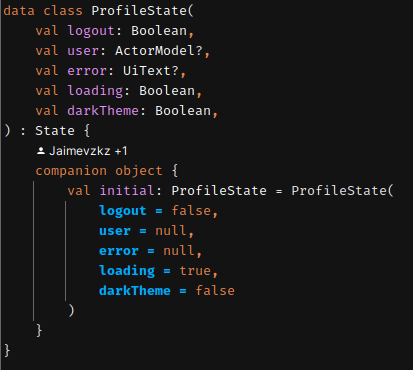
\includegraphics[width = 0.5\textwidth]{Imagenes/Fuentes/ejemplo_estado.png}
        \caption{Ejemplo de estado.}
        \label{fig:ejemplo_estado}
    \end{figure}
    \item \textbf{View}: se encarga de observar el estado y renderizar la vista de forma reactiva. Por ejemplo, en el caso de observar que cambia el valor de la variable loading, dibujaríamos un shimmer (pantalla de carga), cuando el valor de loading se pusiera a \textit{true} y tras comprobar que no hubiera errores, se dibujaría la vista como tal. Esto hace que la vista sea ‘tonta’ en el sentido de que no tiene que tomar ningún tipo de decisión, solo recibe unos datos en el estado y los pinta.
    \item \textbf{Intent}: se define como una acción (No confundir con la clase Intent de Android\hyperlink{cap:biblio}{\endnote{\textbf{Intent}: \url{https://developer.android.com/guide/components/}}}) que se lanza cuando el usuario realiza una acción (o el sistema solicita un cambio de estado). Estas acciones se procesan en un \textit{pipe} del viewmodel y van sobreescribiendo el estado. Es la forma que tiene la vista de cambiar los datos, cuando el usuario realiza una acción (como por ejemplo pulsar un botón), la vista lanza un \textit{intent} que se procesa, haciendo los cambios de estado necesarios, en la figura \ref{fig:ejemplo_intent} se muestran los \textit{intents} declarados para la vista de perfil de usuario.
    \begin{figure}[h]
        \centering
        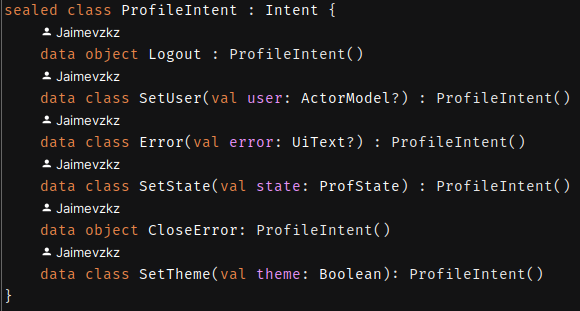
\includegraphics[width = 0.7\textwidth]{Imagenes/Fuentes/ejemplo_intent.png}
        \caption{Ejemplo de definición de los \textit{intents} de una vista.}
        \label{fig:ejemplo_intent}
    \end{figure}
\end{itemize}

Esta estructura define un flujo unidireccional de datos: La vista lanza intents que sobreescriben el estado, como consecuencia de este cambio de estado cambia la vista. Este flujo tiene muchas ventajas que ayudan a crear un código entendible, organizado y escalable. En la figura \ref{fig:visualMvi} se muestra de forma gráfica el ciclo
\hyperlink{cap:biblio}{\endnote{Imagen sacada del articulo publicado por Roberto Fuentes en \textit{Medium}: \href{https://medium.com/@robercoding/qué-es-y-cómo-funciona-la-arquitectura-mvi-desarrollo-android-kotlin-e6a161e1b2db}{\textbf{Fuentes on Medium}}}}.
\begin{figure}[h]
    \centering
    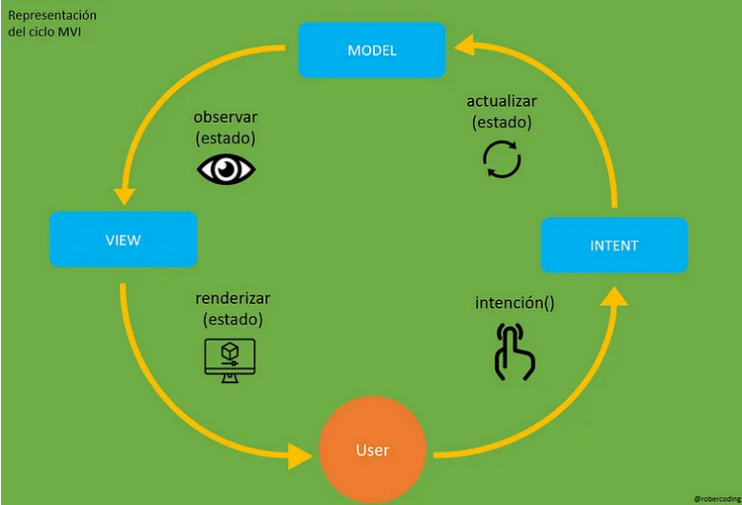
\includegraphics[width = 0.6\textwidth]{Imagenes/Fuentes/visual_mvi.png}
    \caption{Representación gráfica del ciclo MVI.}
    \label{fig:visualMvi}
\end{figure}

\subsection{Principios SOLID}
\label{subsec:solid}
Los principios SOLID son un conjunto de cinco principios de diseño de software que fueron introducidos en el libro \textit{Clean Code} (Martin, 2008)\hyperlink{cap:biblio}{\endnote{\textit{Clean Code: A Handbook of Agile Software Craftsmanship}, Robert C. Martin, 2008}}. Están destinados a guiar a los desarrolladores hacia la creación de código fuente limpio, modular, mantenible y extensible. A continuación se ha descrito brevemente cada uno de ellos, adjuntando una captura del código de la aplicación que lo implementa o una explicación de en qué parte del código se ha implementado cuando lo anterior no sea posible:
\begin{enumerate}
    \item Principio de Responsabilidad Única (\textit{Single Responsibility Principle}): establece que una clase debería tener una única razón para cambiar. En otras palabras, una clase debe tener una sola responsabilidad o función dentro del sistema. En la figura de ejemplo \ref{fig:change_state} se muestra como cualquier clase que implemente la interfaz tendrá la responsabilidad única de implementar el metodo \textit{invoke}.
    \begin{figure}[h]
        \centering
        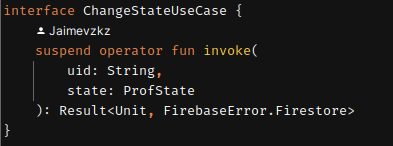
\includegraphics[width = 0.7\textwidth]{Imagenes/Fuentes/change_state.png}
        \caption{Ejemplo de primer principio SOLID.}
        \label{fig:change_state}
    \end{figure}
    \item Principio Abierto/Cerrado (\textit{Open/Closed Principle}): sostiene que las entidades de software (clases, módulos, funciones, etc.) deberían estar abiertas para su extensión pero cerradas para su modificación.
    
    Este principio se podría ver implementado por ejemplo en la funcionalidad \textit{profile}, en la que se podría añadir todo el código que se deseara para añadir funcionalidad sin tener que cambiar nada de lo ya implementado.
    \item Principio de Sustitución de Liskov (\textit{Liskov Substitution Principle}): establece que los objetos de un programa deben ser reemplazables por instancias de sus subtipos sin afectar la integridad del programa.
    
    En Profinder, este principio ha sido implementado por ejemplo en los \textit{viewmodels}, que heredan de la clase \textit{Baseviewmodel}. Cualquier instancia del objeto \textit{Baseviemodel} podría ser sustituido por la implementación de alguna de sus clases hijas sin que cambiara el comportamiento del programa.
    \item Principio de Segregación de la Interfaz (\textit{Interface Segregation Principle}):  sostiene que es mejor el uso de muchas interfaces pequeñas y concretas, mejor que una monolítica para evitar dependencias innecesarias.
    
    Esto se aplica en los casos de uso, cada caso de uso tiene una interfaz específica y concreta.
    \item Principio de Inversión de Dependencias (\textit{Dependency Inversion Principle}): establece que los módulos de alto nivel no deben depender (ni al revés) de los módulos de bajo nivel, ambos deben depender de abstracciones.
    
    Esto se cumple por ejemplo, como se muestra en la figura \ref{fig:ejemplo_reduce}, en la implementación \textit{reduce} de los viewmodel, esta función no tiene ninguna dependecia específica, sino que se adapta a cada caso recibiendo tipos genéricos.
    \begin{figure}[h]
        \centering
        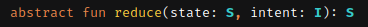
\includegraphics[width = 0.5\textwidth]{Imagenes/Fuentes/ejemplo_reduce.png}
        \caption{Ejemplo del quinto principio SOLID.}
        \label{fig:ejemplo_reduce}
    \end{figure}
\end{enumerate}

\section{Modelo de datos}
\subsection{Descripción detallada}
\begin{itemize}
    \item \textbf{ActorModel}: es la estructura de datos que almacena todos los datos de usuario, se usa la misma tanto para usuarios como para profesionales ya que admite campos nulos para aquellos atributos que solo corresponden a un tipo de actor, en esta estructura se guarda también el tipo de actor, la lista de favoritos (lista con otros \textit{ActorModel}), la calificación y el número de calificaciones tal y como se muestra en la figura \ref{fig:actorModel}.
    \begin{figure}[h]
        \centering
        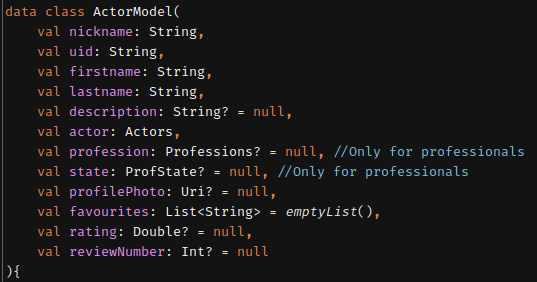
\includegraphics[width = 0.6\textwidth]{Imagenes/Fuentes/actorModel.png}
        \caption{Clase ActorModel.}
        \label{fig:actorModel}
    \end{figure}
    \item \textbf{ServiceModel}: guarda el modelo de un servicio, cuenta con distintos campos como la categoría del servicio, si está activo o no, y el propietario del servicio (un \textit{ActorModel}) tal y como se muestra en la figura \ref{fig:ServiceModel}.
    \begin{figure}[h]
        \centering
        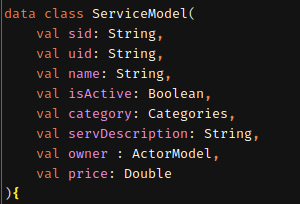
\includegraphics[width = 0.4\textwidth]{Imagenes/Fuentes/ServiceModel.png}
        \caption{Clase ServiceModel.}
        \label{fig:ServiceModel}
    \end{figure}
    \item \textbf{JobModel}: esta clase guarda tanto solicitudes de trabajo como trabajos activos, en un principio se hicieron dos clases separadas para esto, pero se comprobó que la funcionalidad era la misma y se unificó en una sola clase para evitar duplicaciones de código, relacionan el profesional, el usuario y el servicio tal y como se muestra en la figura \ref{fig:JobModel}.
    \begin{figure}[h]
        \centering
        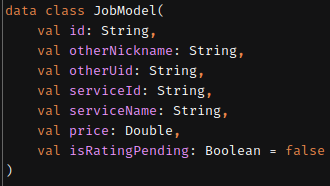
\includegraphics[width = 0.4\textwidth]{Imagenes/Fuentes/JobModel.png}
        \caption{Clase JobModel.}
        \label{fig:JobModel}
    \end{figure}
    \item \textbf{ChatListItemModel}: representa un item en la lista de chats recientes, guarda solo los campos necesarios para mostrar al usuario sin tener que volver a acceder a base de datos para sacar el \textit{ActorModel} completo, tal y como se muestra en la figura \ref{fig:ChatListItemModel}.
    \begin{figure}[h]
        \centering
        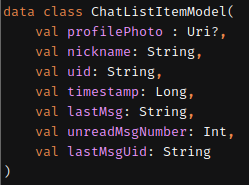
\includegraphics[width = 0.3\textwidth]{Imagenes/Fuentes/ChatListItemModel.png}
        \caption{Clase ChatListItemModel.}
        \label{fig:ChatListItemModel}
    \end{figure}
    \item \textbf{ChatMsgModel}: esta clase representa un mensaje en el chat, guarda el contenido del mensaje, un \textit{timestamp} para saber el momento exacto en el que se envió de cara a ordenarlo en la lista de mensajes, así como para mostrarle la hora al usuario y si el usuario es propietario (lo ha enviado él) o no (lo ha recibido) del mensaje, tal y como se muestra en la figura \ref{fig:ChatMsgModel}.
    \begin{figure}[h]
        \centering
        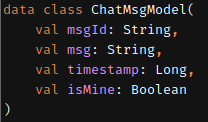
\includegraphics[width = 0.4\textwidth]{Imagenes/Fuentes/ChatMsgModel.png}
        \caption{Clase ChatMsgModel.}
        \label{fig:ChatMsgModel}
    \end{figure}
    \item \textbf{LocationModel}: representa la localización de un usuario, solo guarda los campos que es necesario mostrar en el mapa, la localización y el id del usuario (para poder extraer sus datos si fuera necesario) tal y como se muestra en la figura \ref{fig:LocationModel}.
    \begin{figure}[h]
        \centering
        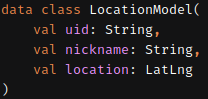
\includegraphics[width = 0.4\textwidth]{Imagenes/Fuentes/LocationModel.png}
        \caption{Clase LocationModel.}
        \label{fig:LocationModel}
    \end{figure}
    \item \textbf{Enums}: También se han usado una serie de enumerados para guardar cosas como los tipos de actores, las categorías de servicios, profesiones, etc. Esto hace que sea muy sencillo añadir nuevos en caso de necesidad sin tener que cambiar código existente, solo añadir nuevo (\textit{Open/Closed Principle}, véase el apartado \ref{subsec:solid}). En la figura \ref{fig:ejemplo_enum} se muestra un ejemplo del enumerado con los tipos de actores.
    
    \begin{figure}[h]
        \centering
        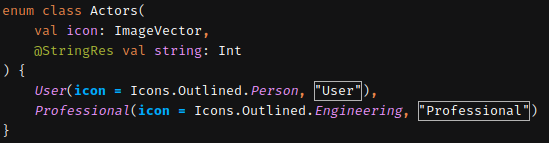
\includegraphics[width = 0.6\textwidth]{Imagenes/Fuentes/ejemplo_enum.png}
        \caption{Ejemplo de enumerado (actores).}
        \label{fig:ejemplo_enum}
    \end{figure}
\end{itemize}

\hypertarget{subsec:firebase}{}
\subsection{Firebase} 
\label{subsec:firebase}
Firebase \hyperlink{cap:biblio}{\endnote{\textbf{Firebase}: \url{https://firebase.google.com/}}} es una plataforma web desarrollada por Google que ofrece una amplia gama de servicios para ayudar a los desarrolladores a crear y mejorar aplicaciones. En Profinder, se ha utilizado como \textit{backend} para toda la aplicación y ha aportado la capacidad de plasmar el modelo de datos de la aplicación a una base datos, así como autenticación y almacenamiento para fotos. A continuación se ha explicado cada servicio utilizado.
\subsubsection{Authentication}
Firebase Authentication\hyperlink{cap:biblio}{\endnote{\textbf{Firebase Authentication}: \url{https://firebase.google.com/docs/auth/}}} es un servicio de autenticación que ahorra todo el proceso de gurdado y cifrado de contraseñas, también gestiona las sesiones de cada usuario, permitiendo mantener la sesión iniciada.Tiene compatibilidad para configurar diversos métodos de autenticación, sin embargo, en esta aplicación solo se ha considerado oportuno implementar la autenticación con \textit{email} y contraseña aunque si se quisiera sería sencillo añadir otros métodos. En la figura \ref{fig:ejemplo_auth} se muestra el panel de control de usuarios en el que se puede realizar un control sobre los mismos (como cambiar contraseñas o suspender cuentas).
\begin{figure}[h]
    \centering
    
\includegraphics[width = 1\textwidth]{Imagenes/Fuentes/ejemplo_auth.png}
    \caption{Captura de pantalla del panel de control de Firebase Authentication.}
    \label{fig:ejemplo_auth}
\end{figure}
\hypertarget{subsec:firestore}{}
\subsubsection{Firestore} 
Firebase Firestore \hyperlink{cap:biblio}{\endnote{\textbf{Firebase Firestore}: \url{https://firebase.google.com/docs/firestore/}}} ha sido la principal base de datos del proyecto, es de tipo no SQL lo cual ha presentado algunas ventajas pero también muchos desafios ya que en este tipo de bases de datos es muy fácil caer en la duplicación de datos y ha sido necesario gastar mucho tiempo en pensar la mejor forma de implementarla. 

En la figura \ref{fig:ejemplo_firestore} se muestra el panel de control de firestore donde se pueden ver, añadir y modificar datos de forma manual. 

La base de datos ha sido dividida en tres colecciones explicadas a continuación (véase el apéndice \ref{Appendix:bd_design} con el diagrama del diseño):
\begin{itemize}
    \item \textbf{users}: cada documento de esta colección se guarda con un id generado automáticamente y es donde se almacenan los datos de cada usuario, así como los \textit{jobs} y \textit{requests}.
    \item \textbf{services}: cada documento de esta colección se guarda con un id generado automáticamente y es donde se almacenan los datos de cada servicio.
    \item \textbf{locations}: cada elemento de esta colección representa la localización de un usuario, se generan con un id igual al id del usuario y guardan el \textit{nickname} a parte de la localización
\end{itemize}
\begin{figure}[h]
    \centering
    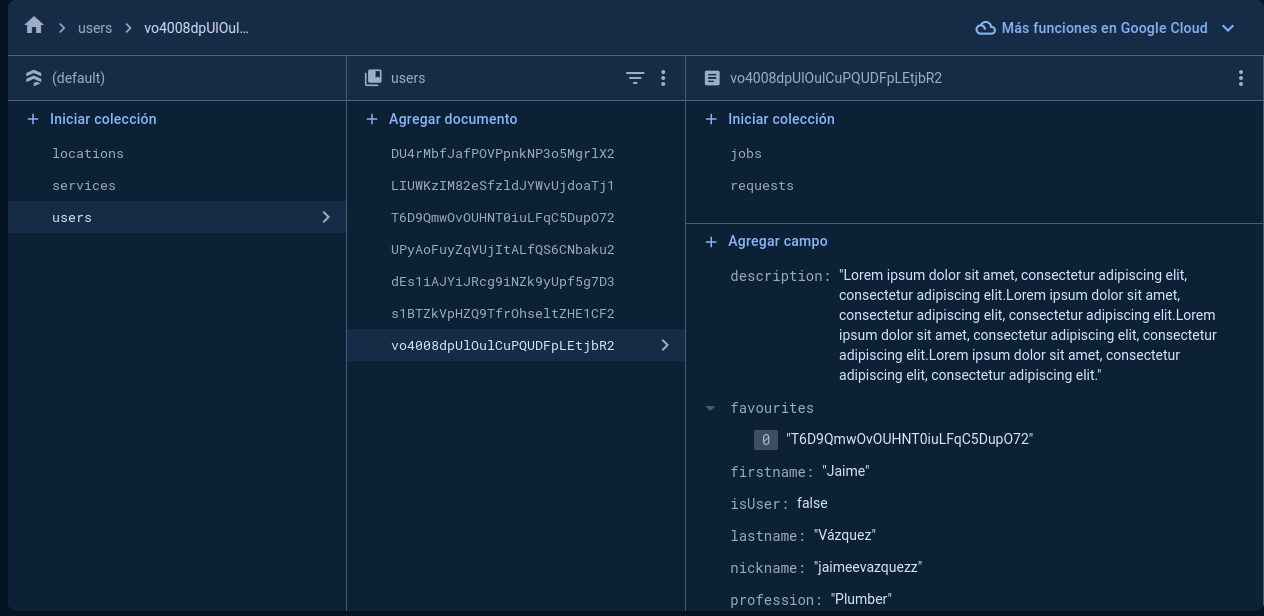
\includegraphics[width = 0.7\textwidth]{Imagenes/Fuentes/ejemplo_firestore.png}
    \caption{Captura de pantalla del panel de control de la base de datos Firestore.}
    \label{fig:ejemplo_firestore}
\end{figure}
\hypertarget{subsec:realtime}{}
\subsubsection{Realtime Database}
Realtime database\hyperlink{cap:biblio}{\endnote{\textbf{Realtime database}: \url{https://firebase.google.com/docs/database/}}} es una base datos de baja latencia, menos sofisticada que \hyperlink{subsec:firestore}{Firestore} pero cuyas funcionalidades han encajado perfectamente con las necesidades del proyecto. Se ha utilizado para toda la funcionalidad de chat ya que al ser los mensajes en tiempo real, era necesario que la latencia fuera mínima. 

En Realtime, los datos se guardan en formato JSON (\textit{JavaScript Object Notation}). Su estructura se ha divido en la lista de chats recientes (conteniendo atributos como el último mensaje, los participantes, la hora y el número de mensajes sin leer por cada conversación entre dos actores de la aplicación) y los chats en sí (conteniendo cada mensaje de una conversación con la hora en que fue mandado). En la figura \ref{fig:ejemplo_realtime} se muestra el panel de control de realtime donde se pueden ver, añadir, eliminar y modificar datos, aunque es menos sofisticado que el panel de control de firestore.
\begin{figure}[h]
    \centering
    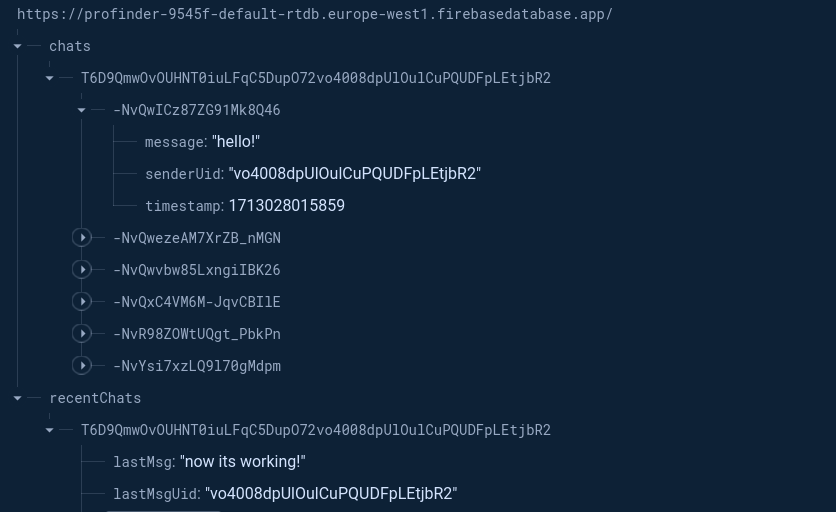
\includegraphics[width = 0.6\textwidth]{Imagenes/Fuentes/ejemplo_realtime.png}
    \caption{Captura de pantalla de la estructura de Realtime Database}
    \label{fig:ejemplo_realtime}
\end{figure}
\subsubsection{Storage}
Firebase storage\hyperlink{cap:biblio}{\endnote{\textbf{Firebase storage}: \url{https://firebase.google.com/docs/storage/}}} es un servicio de alamcenamiento en la nube. Se ha utilizado para almacenar las fotos de perfil de los actores de la aplicacion. Cada foto de perfil se guarda en una carpeta cuyo nombre es el id del actor y se accede a ella a traves de una uri autogenerada que se procesa en la aplicación usando \hyperlink{subsec:coil}{Coil}.

\hypertarget{subsec:datastore}{}
\subsection{Datastore}
Datastore\hyperlink{cap:biblio}{\endnote{\textbf{Datastore}: \url{https://developer.android.com/topic/libraries/architecture/datastore}}} es un sistema de almacenamiento persistente que permite guardar pares clave valor en la aplicación para un acceso rápido a través de 
corrutinas\hyperlink{cap:biblio}{\endnote{\textbf{Corrutinas}: \url{https://developer.android.com/kotlin/coroutines}}} En el caso de Profinder se ha utilizado para guardar 2 cosas:
\begin{itemize}
    \item \textbf{Tema de la aplicación}: de tal forma que cuando se cambia su valor, devuelve un flow\hyperlink{cap:biblio}{\endnote{\textbf{Flows}: \url{https://developer.android.com/kotlin/flow}}} que indica a la Main Activity el tema que debe utilizar. Este tema se mantiene en caché por lo que se podría cerrar la aplicación y al abrirla se recordaría el tema establecido.
    \item \textbf{El id del usuario iniciado}: De tal forma que cuando se necesiten datos del usuario desde cualquier parte de la app se puede conseguir el id (que es único en base de datos) según necesidad, esto servirá para un acceso más rápido en Firestore debido a que es una base de datos que se indexa por este campo.
\end{itemize}

\subsection{Uso del patrón Singleton como modelo de persistencia}
En la programación Android, la persistencia de datos es muy importante ya que al contrario que en otro tipo de programas, cada poco tiempo se borran todos los datos no persistidos para evitar que la aplicación ocupe demasiado espacio en el dispositivo. En este contexto es donde se presenta el problema.

A lo largo del desarrollo de otras aplicaciones (en preparación a esta) se encontró que el uso de una base de datos local suponía una carga de espacio en la aplicación y en tiempo de compilación que la ralentizaba, más allá de esto, las necesidades de Profinder implicaban que los datos fueran actualizados cada no demasiado tiempo puesto que tanto servicios; como favoritos; como los datos de usuario están diseñados para cambiar con frecuencia entre los distintos actores de la aplicación. Por estos motivos se decidió buscar un sistema alternativo que se adecuara a las necesidades de la aplicación: actualización frecuente y poca carga en memoria sin tener que estar accediendo constantemente al servicio remoto (\hyperlink{subsec:firestore}{Firestore}) ya que esto supondría un coste económico.

Esta solución se ha implementado siguiendo el patrón \textit{Singleton}. Los datos a persistir se almacenan en una clase que los guarda de la siguiente forma: si los datos están cacheados los devuelve, si no, los saca del servicio remoto, los cachea y los devuelve. De esta forma la próxima vez que se accedan los datos, estarán cacheados y no hará falta llamar al servicio remoto. La figura \ref{fig:ejemplo_singleton1} muestra la función que implementa la lógica descrita.

\begin{figure}[h]
    \centering
    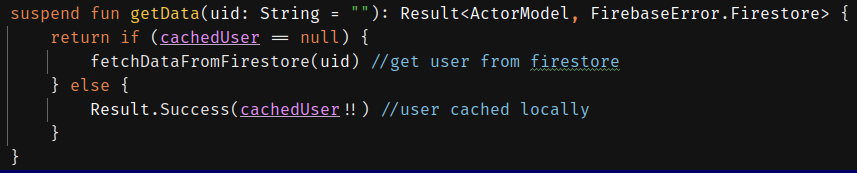
\includegraphics[width = 0.9\textwidth]{Imagenes/Fuentes/ejemplo_singleton1.png}
    \caption{Ejemplo de función getData()}
    \label{fig:ejemplo_singleton1}
\end{figure}

Para acceder a esta función es donde creamos el Singleton (figura \ref{fig:ejemplo_singleton2}) que será accedido desde cualquier lugar donde se necesiten los datos.
\begin{figure}[h]
    \centering
    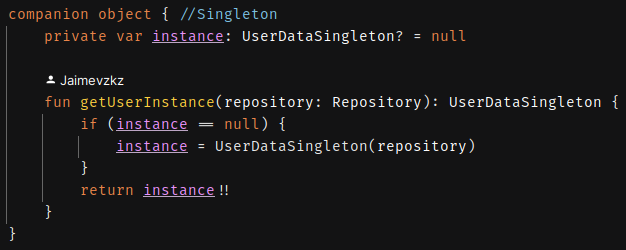
\includegraphics[width = 0.9\textwidth]{Imagenes/Fuentes/ejemplo_singleton2.png}
    \caption{Ejemplo de Singleton con datos de usuario}
    \label{fig:ejemplo_singleton2}
\end{figure}